\chapter{«Build your own tools»: Entwicklung der App Intermind}
\label{sec:entwicklung_app}

% TODO: Sprachlich überarbeiten ich und präsens

Im Rahmen dieser Arbeit habe ich mit der App \gls{intermind} eine Plattform entwickelt, die als technische Grundlage für \gls[noindex]{ema} und \gls[noindex]{gema}-Befragungen dient. Die App und der in dieser Arbeit eingesetzte Fragenkatalog wurden parallel und iterativ konzipiert. Während ich in diesem Kapitel die technische Entwicklung der App dokumentiere, erläutere ich die inhaltliche Gestaltung des Fragebogens im \cref{sec:fragebogenentwicklung}. 

Der vollständig dokumentierte Quellcode der App ist auf \gls[noindex]{github}\footnote{\href{https://github.com/lbatschelet/InterMind}{https://github.com/lbatschelet/InterMind}} unter einer \gls{lic:agpl}-Lizenz veröffentlicht.


\section{From Scratch -- Warum eine eigene App?}
\label{sec:entwicklung_app_begruendung}

Um die Fragestellung dieser Arbeit zu bearbeiten, wird eine Plattform benötigt, welche wiederholte, geolokalisierte und kontextsensitive Erhebungen im Alltag der Teilnehmenden ermöglicht. Naheliegend wäre der Rückgriff auf bestehende und in Forschung eingesetzte Plattformen wie \gls{urbanmind}. Wie in \cref{sec:vergleich_bestehender_instrumente} beschrieben, ist diese App aber nicht vollständig nachvollziehbar noch eigenständig anpassbar. Insbesondere bei der Erhebung sensibler Daten zu (Un-)Wohlbefinden, sozialen Positionierungen und erlebter Diskriminierung ist eine transparente, kontrollierbare und sichere Datenverarbeitung jedoch essenziell.

Auch kommerzielle Lösungen wie die Marktforschungsplattform \textit{Avicenna}\footnote{\href{https://avicennaresearch.com/}{https://avicennaresearch.com/}} kommen nicht infrage -- neben hohen Lizenzkosten bieten auch sie nur eingeschränkte Anpassungs- und Kontrollmöglichkeiten und erfüllen zentrale ethische Anforderungen nicht.

Aus dieser Analyse ergibt sich die Notwendigkeit, ein eigene Plattform zu entwickeln, die diesen Anforderungen gerecht wird. Sie soll mobil und einfach nutzbar sein, Antworten im situativen Alltag der Teilnehmenden ermöglichen und Standortdaten automatisch erfassen. Dabei sollen bestmögliche Datenschutz-Standards eingehalten und technische Hürden möglichst gering gehalten werden. Gleichzeitig soll sie so flexibel und nachhaltig gestaltet sein, dass Fragenkataloge, Inhalte und Erhebungslogik für zukünftige Arbeiten mit nur kleinem Aufwand angepasst werden können.

Die Entscheidung zur Entwicklung einer eigenen Erhebungs-Plattform ist nicht nur technisch motiviert, sondern folgt auch einer forschungsethischen Logik: Wie im \cref{sec:datafeminism} dargelegt, sind digitale Infrastrukturen nie neutral, sondern Ausdruck gesellschaftlicher Machtverhältnisse. Eine transparente und kontrollierbare Datenverarbeitung ist insbesondere dann zentral, wenn -- wie im vorliegenden Projekt -- sensible Informationen zu Wohlbefinden, sozialer Zugehörigkeit und Diskriminierung erhoben werden. Ich verstehe vor diesem Hintergrund die Entscheidung für eine \gls[noindex]{opensource}-Architektur als Ausdruck eines bewussten Gestaltungswillens im Sinne digitaler Souveränität: Die gesamte Infrastruktur soll nachvollziehbar, anpassbar und kollektiv weiterentwickelbar bleiben, um technologische Gestaltungsmacht nicht an proprietäre Systeme abzugeben, sondern sie partizipativ zurückzugewinnen.

\section{Konzeption und Anforderungen -- Der Weg zur eigenen Infrastruktur}
\label{sec:app_entwicklung_anforderungen}

In einem ersten Schritt entwickle ich auf Basis der grob beschriebenen Anforderungen zunächst einen detaillierten Anforderungskatalog, der als zentraler Leitfaden für die weiteren Schritte der Entwicklung dient. Dieser Katalog wird im gesammten Entwicklungsprozess iterativ ergänzt, konkretisiert und kontinuierlich an methodische und technische Erkenntnisse angepasst. Die Klassifikation der Anforderungen erfolgt orientiert an der in der Softwareentwicklung üblichen Unterscheidung zwischen funktionalen und nicht-funktionalen Anforderungen.

Funktionale Anforderungen definieren konkret, \textit{was} die App leisten muss, und legen somit die notwendigen Funktionen und Abläufe der Anwendung fest. Für diese Anwendung bedeutet dies insbesondere, dass die App den Teilnehmenden täglich mehrere zufällig verteilte Zeitfenster zur Beantwortung von Fragen ermittelt und jeweils zu Beginn dieser Zeiträume \glspl{pushnotification} sendet. Da gängige Webbrowser keine verlässlichen Push-Benachrichtigungen oder zeitgesteuerten Hintergrundprozesse erlauben, schliesst diese Anforderung eine browserbasierte Erhebung aus und führt zur Entscheidung für eine App-basierte Lösung. Um die Erhebung flexibel und bedarfsgerecht zu gestalten, unterstützt sie verschiedene Fragetypen -- darunter Single-Choice, Multiple-Choice, Skalen-basierte Fragen (Slider) sowie Freitextfelder und erhebt zusätzlich bei jeder Befragung automatisiert den aktuellen \gls{gps}-Standort. Im Sinne der Selbstbestimmung über die eigenen Daten ist es funktional zwingend vorgesehen, dass Teilnehmende sämtliche mit ihrem Gerät verknüpften Daten eigenständig und dauerhaft löschen können. Die Teilnahme erfolgt vollständig pseudonym, ohne dass eine Registrierung oder die Angabe personenbezogener Daten erforderlich ist. Darüber hinaus muss die App auf \gls{android}- und \gls{ios}-Geräten lauffähig sein, in Deutsch, Englisch und Französisch verfügbar sein und die Möglichkeit zur Erweiterung um weitere Sprachen bieten. Eine ursprünglich geplante Offlinefähigkeit wird im Verlauf der Entwicklung verworfen, da sie zu Inkompatibilitäten bei der Aktualisierung des Fragenkatalogs führt.

Nicht-funktionale Anforderungen legen fest, \textit{wie} die oben beschriebenen Funktionen umgesetzt werden sollen, und beschreiben qualitative Merkmale wie Sicherheit, Benutzerfreundlichkeit oder technische Nachvollziehbarkeit. Zu den zentralen nicht-funktionalen Anforderungen zählen Datenschutz, Datensicherheit und technische Qualität. Sämtliche Datenverarbeitungsprozesse müssen im Einklang mit dem Schweizer Datenschutzgesetz (\glsxtrshort{dsg}) sowie der Europäischen Datenschutzgrundverordnung (\glsxtrshort{dsgvo}) erfolgen. Wo möglich verwende zusätzlich ich erweiterte Datenschutzstandards. Diese Ausgestaltung folgt nicht nur rechtlichen Vorgaben, sondern knüpft auch an die im \cref{sec:datafeminism} entwickelten Prinzipien einer digitalen Souveränität an, die Transparenz, Kontrolle und Selbstbestimmung in den Mittelpunkt stellt. Eine offene, modulare und nachvollziehbare Codebasis soll gewährleisten, dass Anpassungen und Erweiterungen des Systems durch andere Forschende mit minimalem Aufwand möglich sind. Dies wurde durch die Veröffentlichung der App als \gls{opensource}-Projekt auf \gls{github} umgesetzt.

Zur systematischen Umsetzung der Anforderungen wird ein iterativer Entwicklungsprozess auf Basis von \glspl{githubissue} genutzt, in dem jede funktionale und nicht-funktionale Anforderung als eigenes \glslink{githubissue}{Issue} dokumentiert und mit einem Meilenstein versehen ist, der den geplanten Umsetzungszeitpunkt markiert. Diese Meilensteine orientieren sich an vier Entwicklungsstufen: Als \textit{core \glsxtrfull{mvp}} wird die minimal funktionsfähige Version der App bezeichnet, die alle für die Durchführung der Studie zwingend notwendigen Funktionen enthält, wie etwa die zeitgesteuerte Versendung von \glspl{pushnotification}, die Erfassung des \gls{gps}-Standorts oder die Bereitstellung zentraler Fragetypen. Das \textit{extended \gls{mvp}} umfasst zusätzliche Funktionen, die den Erhebungsprozess verbessern, für die Beantwortung der Forschungsfragen jedoch nicht zwingend erforderlich sind, beispielsweise die Unterstützung mehrerer Sprachen oder zusätzliche Fragetypen. Der Meilenstein \textit{app store release} umfasst alle Aufgaben, die für die Veröffentlichung in App-Stores erforderlich sind, jedoch keinen direkten Einfluss auf die eigentliche Datenerhebung oder Kernfunktionen der App haben. Dazu zählen begleitende Arbeiten wie die Erstellung einer Projektwebsite mit Datenschutzrichtlinie, die Bereitstellung der für die App-Store-Einreichung notwendigen Assets, die Einrichtung einer kontinuierlichen Integrations- und Auslieferungspipeline (\gls{cicd}) sowie die Durchführung des formalen Prüf- und Freigabeprozesses der App-Stores. Unter \textit{future enhancements} werden schliesslich langfristig geplante Erweiterungen verstanden, die den Funktionsumfang der App über die Anforderungen der vorliegenden Arbeit hinaus erweitern. Für die Priorisierung innerhalb dieser Kategorien orientiere ich mich an den Forschungszielen, den rechtlichen Vorgaben, der technischen Machbarkeit innerhalb des vorgegebenen zeitlichen Rahmens sowie an den in \cref{sec:datafeminism} ausgeführten Prinzipien, wobei ich Änderungen am Funktionsumfang während der Entwicklung fortlaufend in den entsprechenden \glslink{githubissue}{Issues} dokumentiere.


\section{Technische Umsetzung -- Prinzipien, Praktiken und Kompromisse}
\label{sec:app_entwicklung_technische_umsetzung}

Für die technische Umsetzung folge ich etablierten Prinzipien der Softwareentwicklung, insbesondere \textit{Privacy by Design} \parencite{cavoukianPrivacyDesign72009} und den Gestaltungsprinzipien von \gls{solid} \parencite{martinCleanArchitectureCraftsmans2018}. Ziel ist eine modulare, wartbare und erweiterbare Architektur, die funktionale Anforderungen effizient umsetzt und nicht-funktionale Anforderungen -- insbesondere Datenschutz und Sicherheit -- von Beginn an integriert. Dabei wird eine klare Trennung zwischen Anwendungslogik, Datenhaltung und Benutzeroberfläche konsequent umgesetzt, um spätere Anpassungen und Erweiterungen mit minimalem Eingriff in bestehende Komponenten zu ermöglichen.

Für die Entwicklung der mobilen Anwendung verwende ich \gls{reactnative} in Kombination mit \gls{expo}. \gls{reactnative} ist ein von \gls{meta} entwickeltes, \gls{opensource} \gls{framework}, das die Entwicklung plattformübergreifender Anwendungen mit einer einzigen Codebasis ermöglicht. Dadurch können \gls{ios}- und \gls{android}-Versionen parallel gepflegt werden, was den Entwicklungs- und Wartungsaufwand erheblich reduziert. Obwohl React Native ursprünglich von \gls{meta} entwickelt wird, erfolgt in diesem Projekt keinerlei Datenaustausch mit dem Konzern, da ausschliesslich das in der Entwicklungsumgebung installierte Framework verwendet wird, das weder auf den Endgeräten der Teilnehmenden noch auf externen Servern von \gls{meta} ausgeführt wird.

\gls{expo} ergänzt React Native um eine ebenfalls \gls{opensource} integrierte Entwicklungsumgebung mit Werkzeugen für Build, Test und Veröffentlichung. Dies erlaubt es, zentrale Infrastrukturaufgaben ohne eigenes \gls{devops}-Team effizient umzusetzen. Insbesondere die Möglichkeit, native Funktionen wie Push-Benachrichtigungen, Kamera- oder Standortzugriff über ein einheitliches API zu nutzen, beschleunigt die Umsetzung und reduziert die Komplexität der Codebasis.

Als serverseitige Infrastruktur verwende ich \gls{supabase} -- ein \gls{opensource} \gls{backend}-as-a-Service auf Basis von \gls{postgresql}, das Authentifizierung, Autorisierung, Datenspeicherung und Schnittstellenbereitstellung integriert. Die Entscheidung für Supabase erfolgt bewusst gegen den Einsatz von \gls{firebase}, das als De-facto-Standard für mobile Anwendungen gilt und in vielen Bereichen eine einfachere Implementierung ermöglicht. Firebase ist jedoch ein proprietärer Dienst von \gls{google}, der zentrale Kontrolle über die Infrastruktur ausübt, den Serverstandort nicht frei wählen lässt und die Datenhoheit einschränkt. Wie in \cref{sec:datafeminism} ausgeführt, stehen solche zentralistischen Strukturen im Widerspruch zu Prinzipien digitaler Souveränität. Supabase ermöglicht hingegen, den Standort des Servers (hier: Schweiz) festzulegen und bietet zusätzlich die Option eines vollständig selbstverwalteten und gehosteten Betriebs. Neben der offenen Lizenz und der \gls{tech:sql}-basierten Datenstruktur ist auch die Möglichkeit eines kostenlosen Hostings für kleine Projekte ausschlaggebend, wodurch der Betrieb ohne zusätzliche Infrastrukturkosten möglich ist. Die Wahl dieser Toolchain stellt damit einen pragmatischen Kompromiss dar: Sie bietet die notwendige technische Leistungsfähigkeit und Flexibilität, ohne die Kontrolle über Daten an externe Plattformanbieter abzugeben.

\begin{figure}[h]
    \centering
    \begin{minipage}[t]{0.38\textwidth}
        \centering
        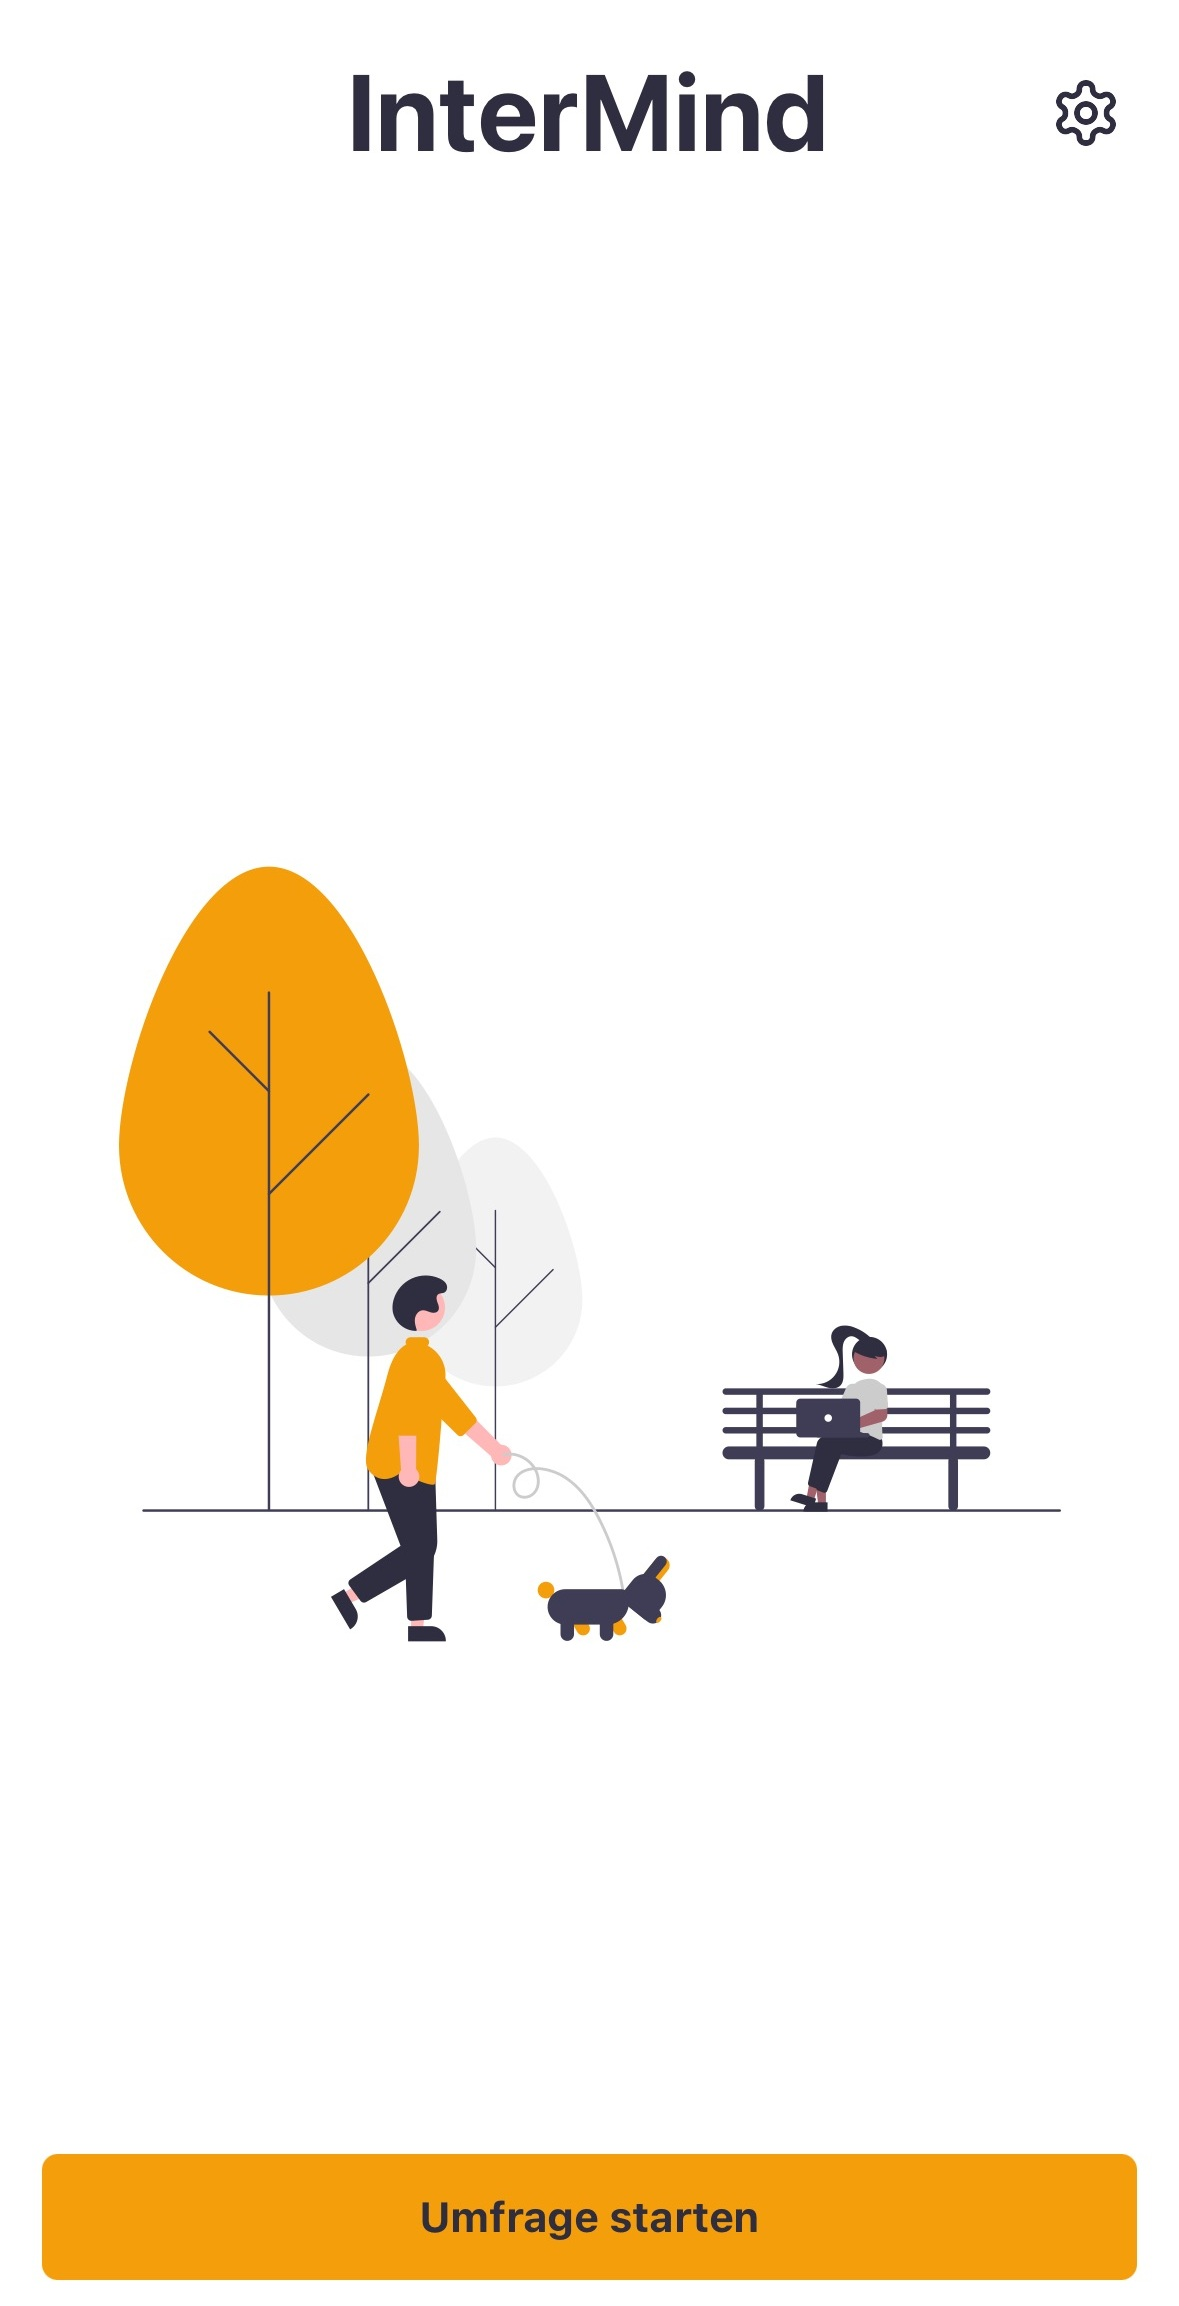
\includegraphics[width=\textwidth]{Arbeit/Bilder/printscreens/startscreen.jpeg}
        \caption{Startbildschirm der App \gls[noindex]{intermind}}
        \label{fig:startscreen}
    \end{minipage}
    \hspace{0.1\textwidth}
    \begin{minipage}[t]{0.38\textwidth}
        \centering
        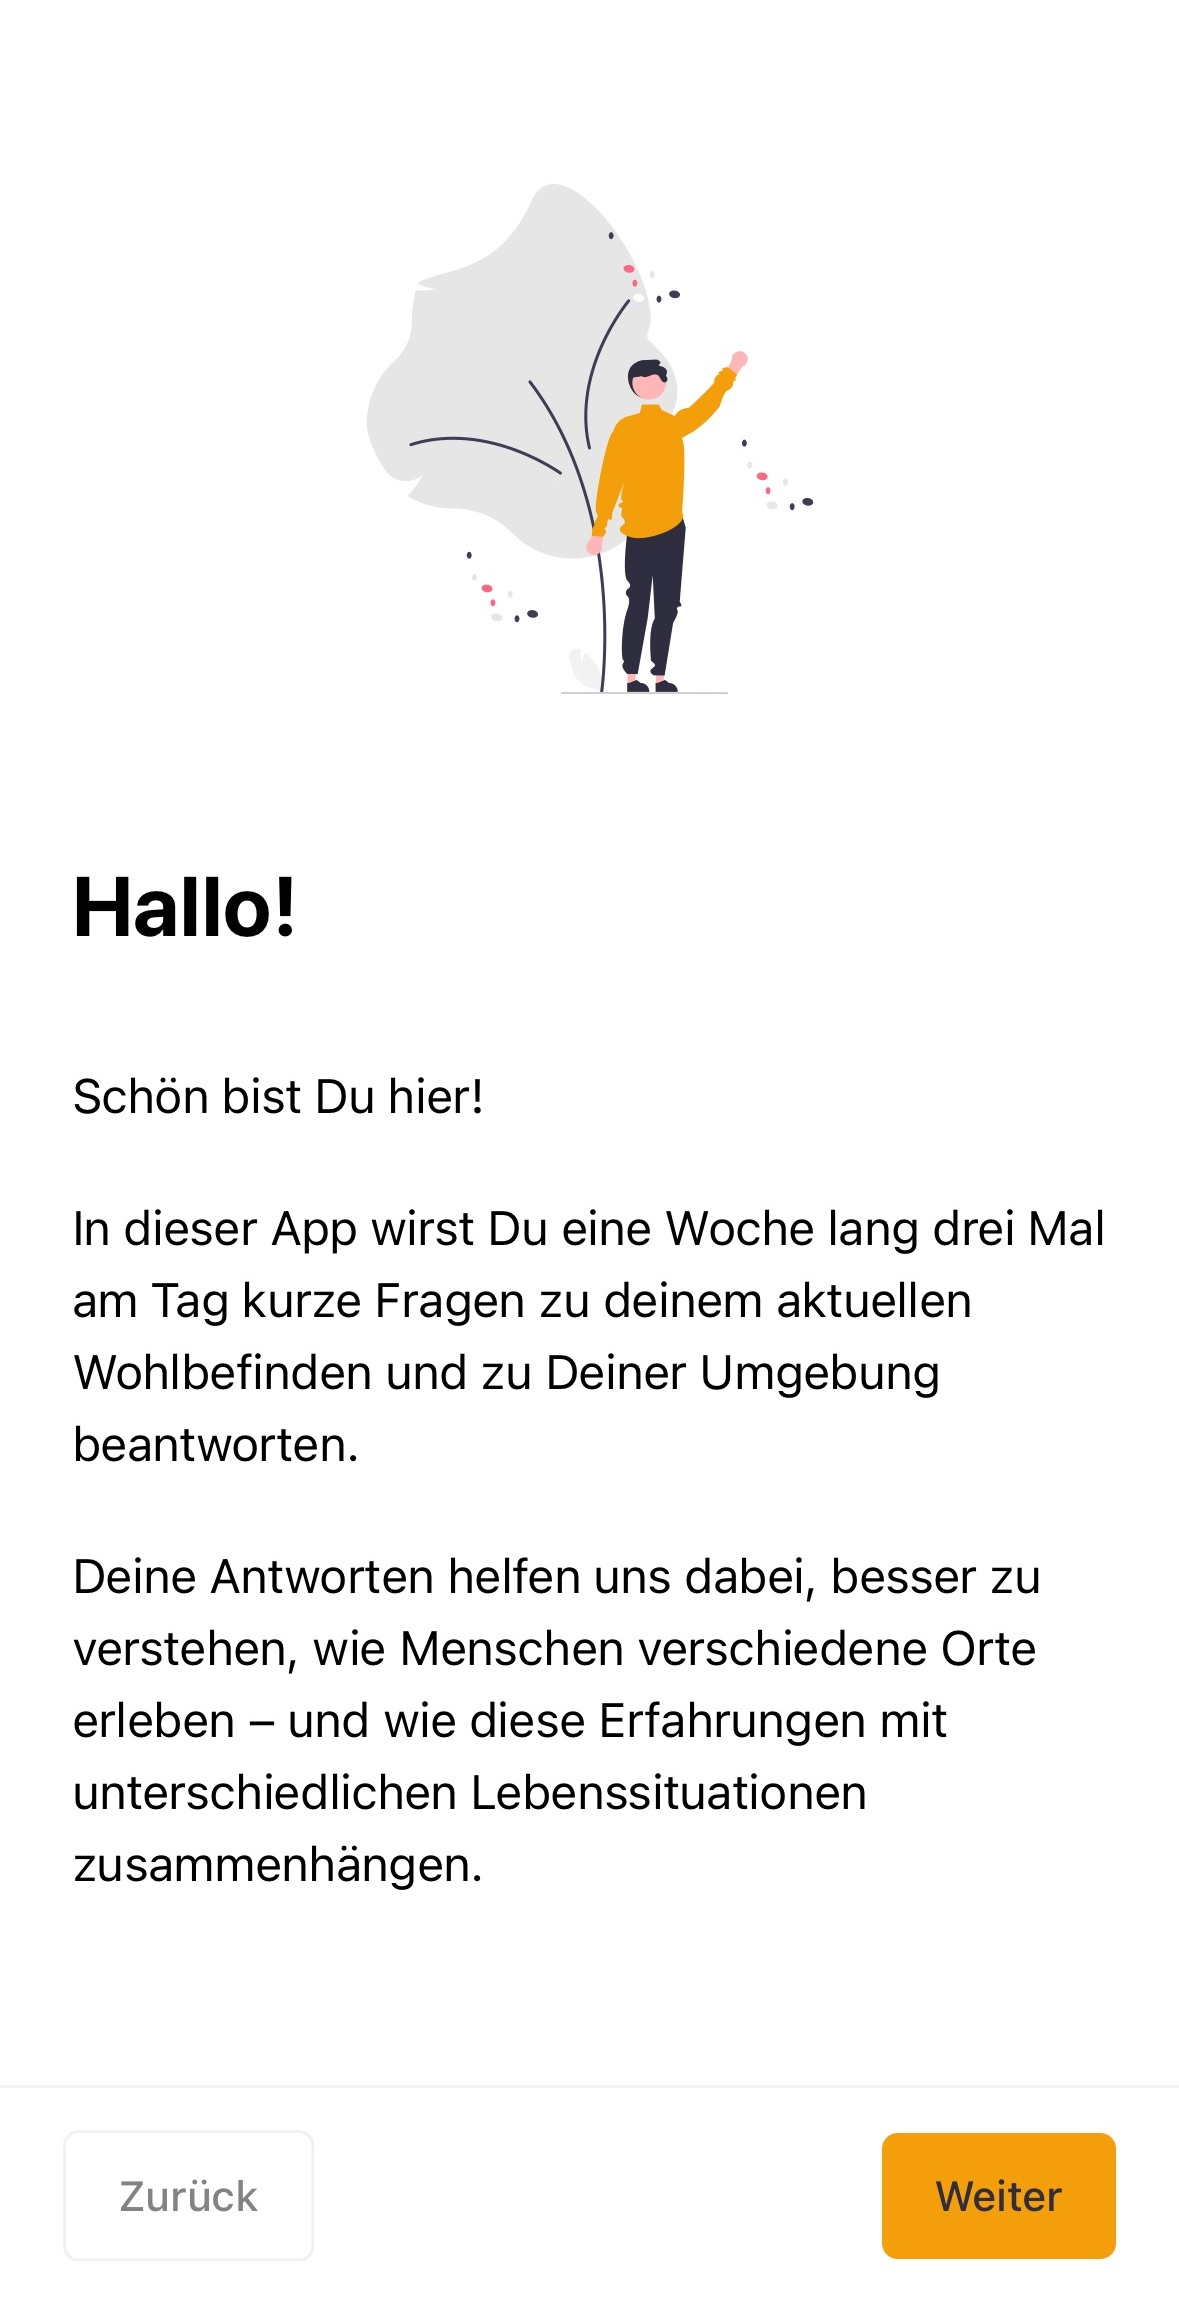
\includegraphics[width=\textwidth]{Arbeit/Bilder/printscreens/welcome.jpeg}
        \caption{Begrüssungstext der App \gls[noindex]{intermind}}
        \label{fig:welcome}
    \end{minipage}
\end{figure}

Der Quellcode folgt einer komponentenbasierten Struktur, in der jede Funktion klar abgegrenzte Verantwortlichkeiten besitzt. Diese Struktur erleichtert die Wiederverwendung bestehender Module für künftige Erweiterungen. Die konkreten Fragebögen (\gls[noindex]{vgl} \cref{sec:fragebogenentwicklung}) werden nicht im Quellcode gespeichert, sondern als \gls{json}-Konfigurationsdateien in der \gls{tech:db} hinterlegt. Die App lädt diese Inhalte dynamisch beim Start oder bei Bedarf nach, wodurch Änderungen am Fragenkatalog ohne App-Update möglich sind. Die Entscheidung für serverseitige Speicherung erhöht die Flexibilität, birgt jedoch den Nachteil, dass eine aktive Internetverbindung erforderlich ist. Auf eine vollständige Offlinefähigkeit wird bewusst verzichtet, um Inkonsistenzen zwischen verschiedenen App-Versionen zu vermeiden und stets aktuelle Inhalte bereitzustellen.

Die datenschutzbezogene Umsetzung basiert auf einer strikten Pseudonymisierung. Beim ersten Start generiert die App automatisch eine gerätegebundene \gls{uuid}, die für alle weiteren Interaktionen verwendet wird. Aus Sicht des Systems existieren damit keine individuellen Nutzer\genderstern innen, sondern ausschliesslich Geräte-IDs. Personenbezogene Daten wie Name, Telefonnummer oder E-Mail-Adresse werden nicht erhoben. Standortdaten werden ausschliesslich zum Zeitpunkt einer beantworteten Befragung erfasst. Die Löschung aller mit einer \gls{uuid} verknüpften Datensätze kann jederzeit direkt in der App ausgelöst werden und entfernt sämtliche Einträge aus der \gls{tech:db}.

Der Zugriffsschutz der \gls{tech:db} auf \gls{supabase} wird durch eine Zugriffskontrolle auf Zeilenebene (\gls{rls}) in der \gls{postgresql}-\gls{tech:db} realisiert. Jede Anfrage an den Server ist an die jeweilige \gls{uuid} gebunden; Abfragen liefern nur Datensätze, die mit dieser ID verknüpft sind. Alle Datenübertragungen zwischen App und Server erfolgen verschlüsselt über authentifizierte Schnittstellen. Die Serverinfrastruktur befindet sich physisch in der Schweiz und unterliegt damit dem Schweizer Datenschutzgesetz (\gls{dsg}); zusätzlich werden die Vorgaben der Europäischen Datenschutzgrundverordnung (\gls{dsgvo}) eingehalten. Die vollständigen Regelungen sind in einer öffentlich zugänglichen Datenschutzrichtlinie dokumentiert, die in der App sowie auf der Projektwebseite\footnote{\href{https://intermind.ch/privacy-policy.html}{https://intermind.ch/privacy-policy.html}} verfügbar ist.

\begin{figure}[h]
    \centering
    \begin{minipage}[t]{0.38\textwidth}
        \centering
        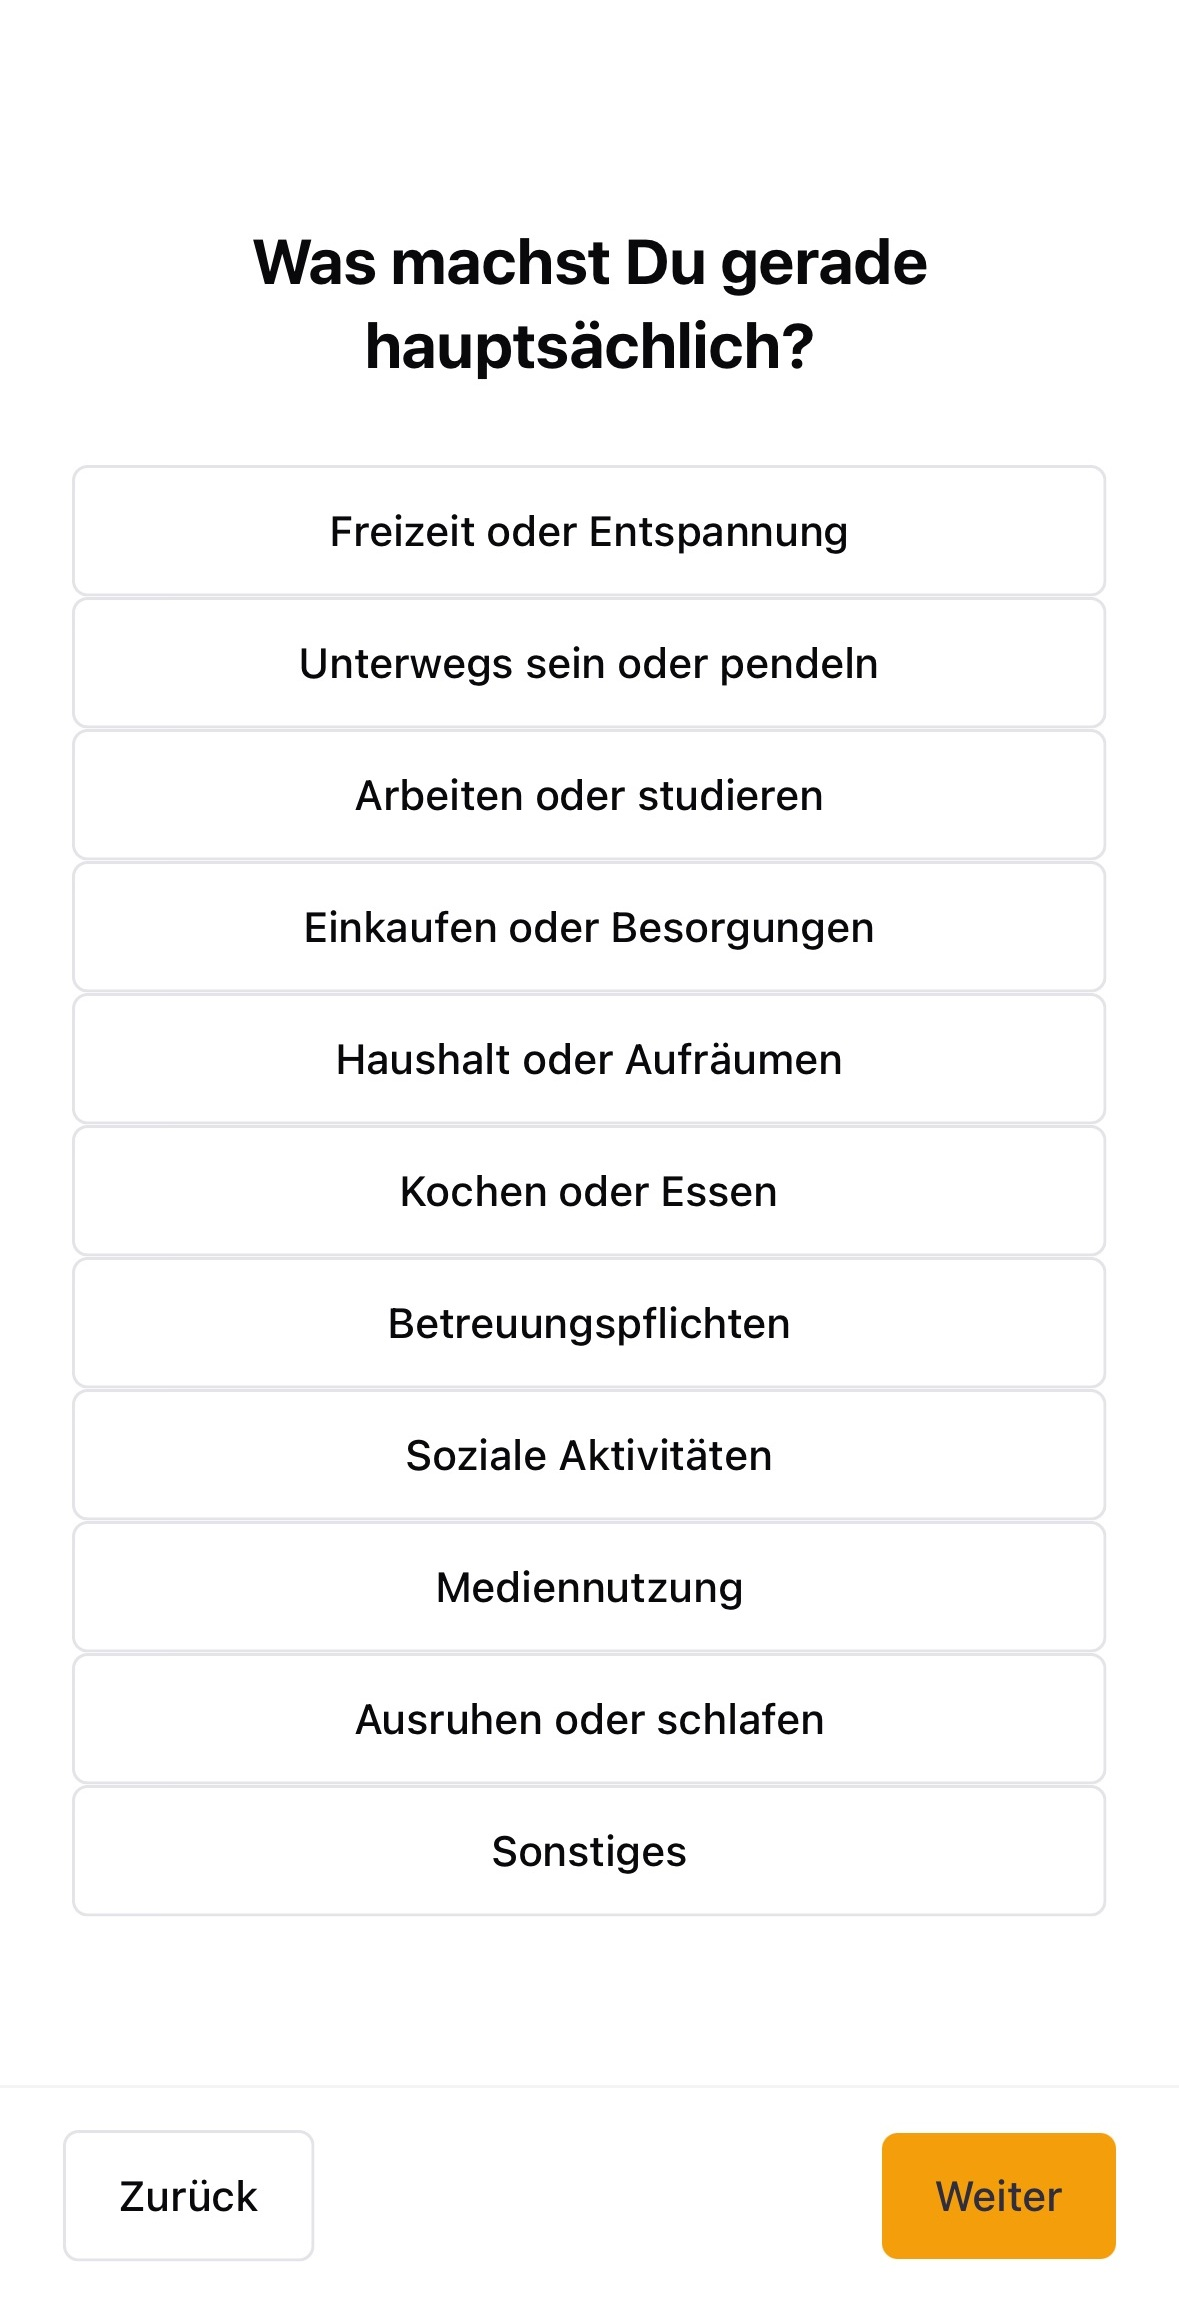
\includegraphics[width=\textwidth]{Arbeit/Bilder/printscreens/beschaeftigung.jpeg}
        \caption{Multiple-Choice-Frage zur aktuellen Beschäftigung}
        \label{fig:beschaeftigung}
    \end{minipage}
    \hspace{0.1\textwidth}
    \begin{minipage}[t]{0.38\textwidth}
        \centering
        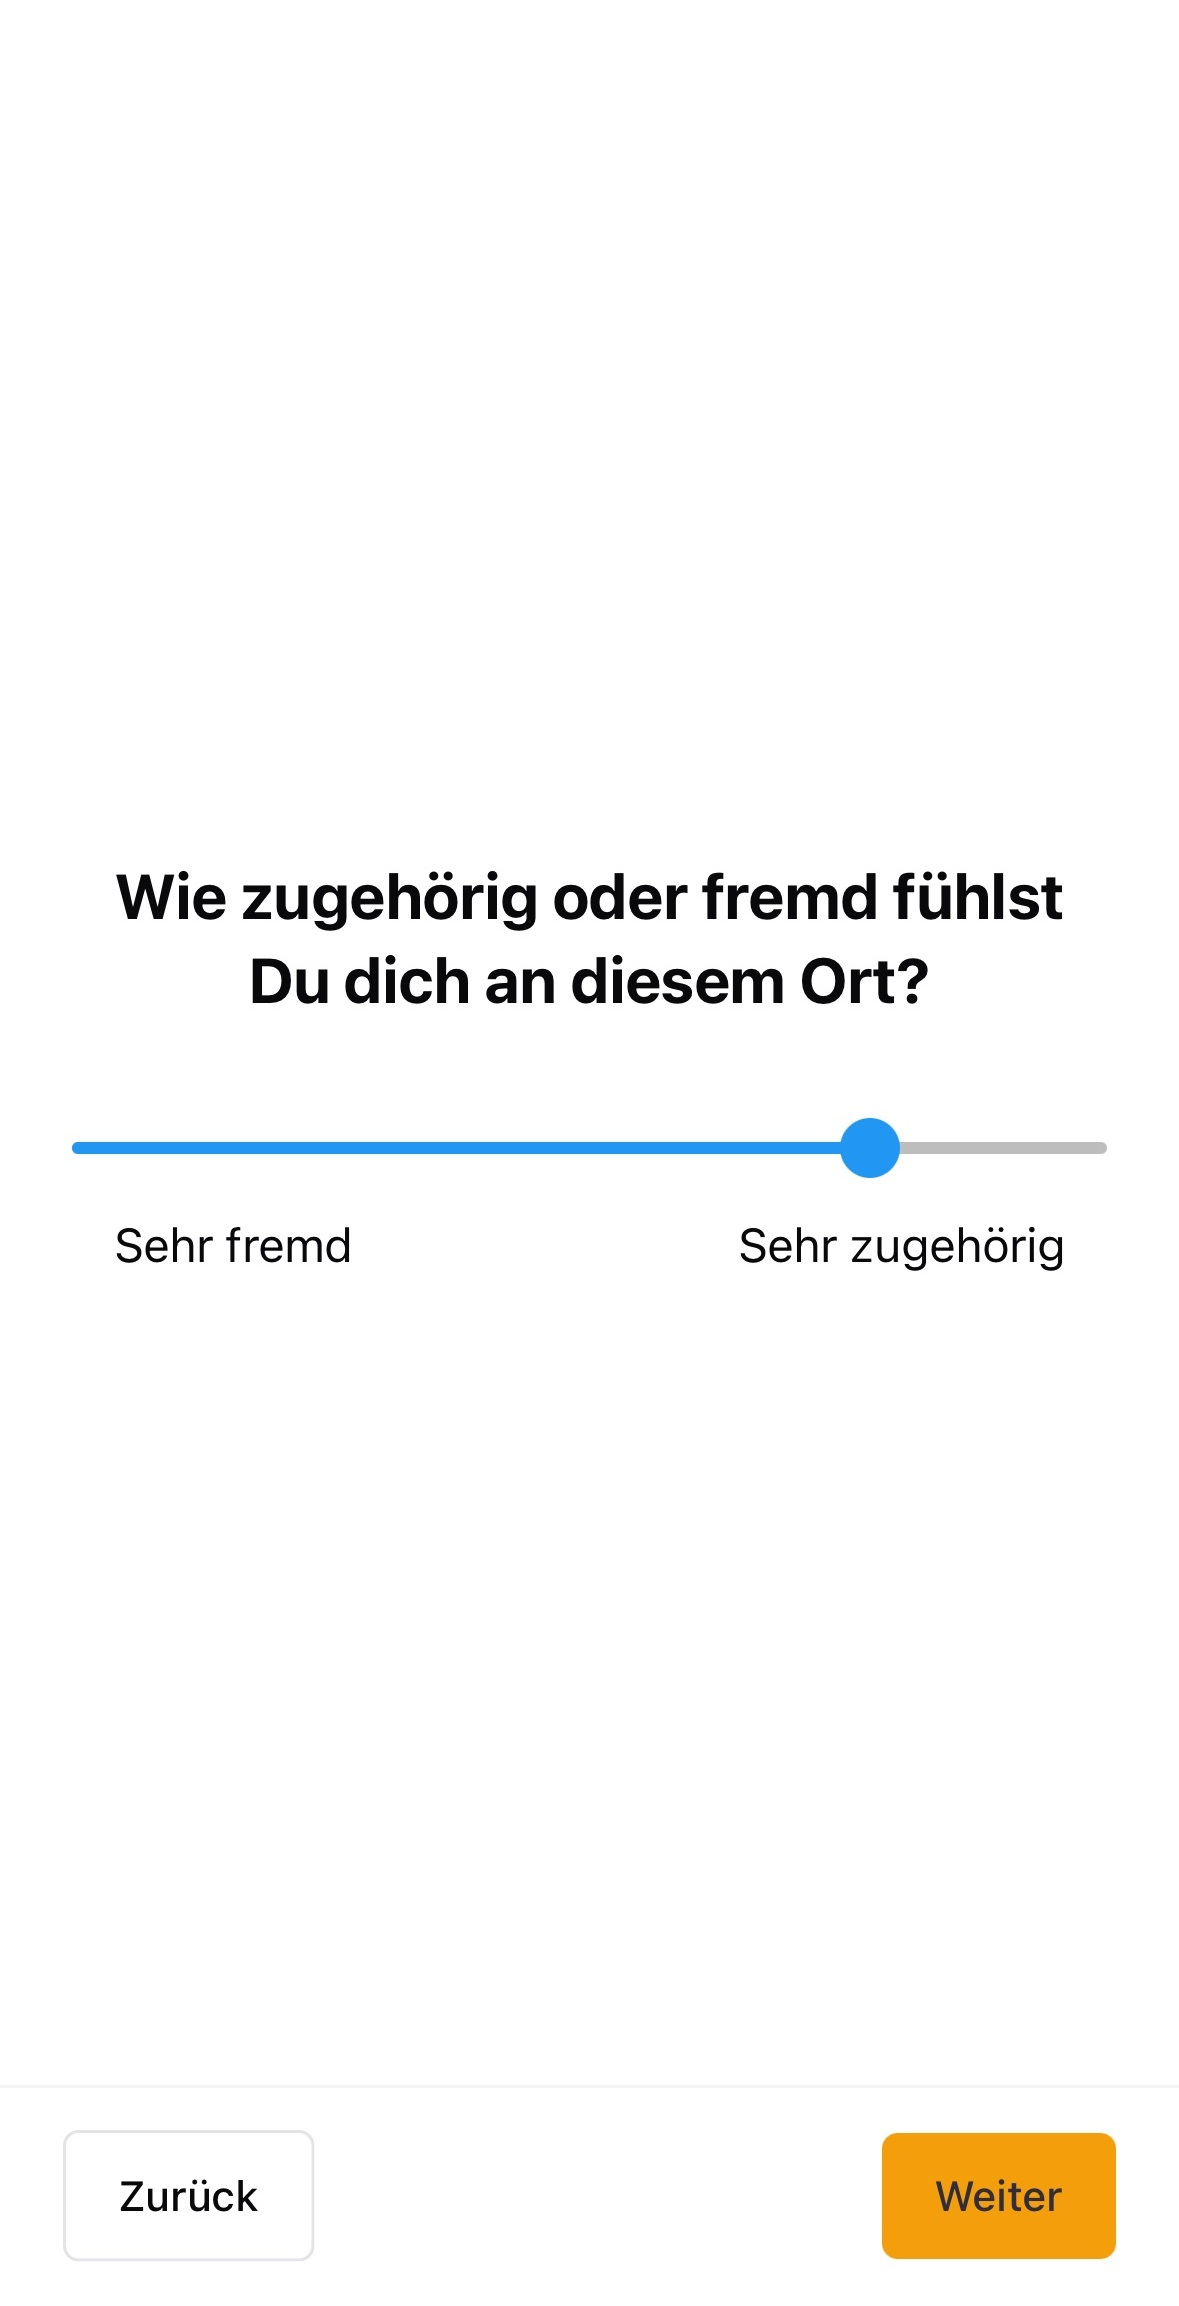
\includegraphics[width=\textwidth]{Arbeit/Bilder/printscreens/zugehoerigkeit.jpeg}
        \caption{Slider-Frage zur sozialen Zugehörigkeit}
        \label{fig:zugehoerigkeit}
    \end{minipage}
\end{figure}

Die App berechnet nach der ersten Teilnahme für den ganzen Befragungszeitraum täglich drei zufällige Befragungszeitpunkte, die innerhalb fester Tagesabschnitte (Morgen, Mittag/Nachmittag, Abend) ausgewählt werden. Diese Zeitpunkte werden lokal auf dem Gerät gespeichert. Zwischen zwei Befragungen wird ein Mindestabstand von zwei Stunden eingehalten, gerechnet zwischen dem Ende des vorigen und dem Beginn des nächsten Befragungsfensters, um zu vermeiden, dass Teilnehmende bei kurzfristiger Nichtverfügbarkeit mehrere Erhebungen unmittelbar hintereinander verpassen. Zum Start eines Zeitfensters wird eine Push-Benachrichtigung versendet; der Fragebogen kann innerhalb einer Stunde beantwortet werden, danach verfällt der Slot.

Die Entscheidung für dieses Zeitplanmodell orientiert sich am Design der \textit{Urban Mind}-App \parencite{bakolisUrbanMindUsing2018}, das sich in mehreren von mir durchgeführten Tests als gut umsetzbar erwiesen hat. Die Kombination aus zufälliger Platzierung der Startzeiten innerhalb fest definierter Tagesfenster und einer begrenzten Bearbeitungsdauer ermöglicht es, Antworten zu unterschiedlichen Zeitpunkten des Tages zu erfassen und damit Variabilität im Tagesablauf der Teilnehmenden abzubilden. Gleichzeitig wird vermieden, dass Befragungen immer zu denselben Uhrzeiten stattfinden, was potenzielle Antwortmuster verzerren könnte.

Die Eckzeiten der drei Hauptzeitfenster sind als Variablen in der Anwendung hinterlegt und können für andere Studien oder Fragebogendesigns angepasst werden. Auf diese Weise lässt sich der Befragungsrhythmus flexibel anpassen, beispielsweise indem Tagesfenster auf Grundlage individueller Angaben zu Aufsteh- und Schlafenszeiten definiert werden. Eine solche Erweiterung würde auch nicht-normative Tagesrhythmen berücksichtigen und könnte die Erreichbarkeit der Teilnehmenden weiter verbessern.

\begin{figure}[h]
    \centering
    \begin{minipage}[t]{0.38\textwidth}
        \centering
        
\includegraphics[width=\textwidth]{Arbeit/Bilder/printscreens/fragen_zu_dir.jpeg}
        \caption{Überleitungsbildschirm zu den einmaligen Fragen}
        \label{fig:ueberleitungsbildschirm}
    \end{minipage}
    \hspace{0.1\textwidth}
    \begin{minipage}[t]{0.38\textwidth}
        \centering
        
\includegraphics[width=\textwidth]{Arbeit/Bilder/printscreens/offen_unwohl.jpeg}
        \caption{Offene Textfrage zu weiteren Gründen für Unwohlsein an diesem Ort}
        \label{fig:offene_textfrage}
    \end{minipage}
\end{figure}

Die Benutzeroberfläche ist bewusst reduziert und funktional gestaltet, um eine intuitive Bedienung zu ermöglichen und die Fragen möglichst neutral darzustellen \parencite{rogersInteractionDesignHumancomputer2023}. Die App umfasst drei Hauptbereiche: den Startbildschirm (\cref{fig:startscreen}), der standardmässig den nächstmöglichen Befragungszeitpunkt prominent anzeigt und -- sofern aktuell eine Befragung verfügbar ist -- direkt einen \enquote{Umfrage starten}-Button einblendet; den Fragebogenbereich (\cref{fig:welcome,fig:beschaeftigung,fig:zugehoerigkeit,fig:ueberleitungsbildschirm,fig:offene_textfrage}), der sowohl einleitende und überleitende Texte als auch die einzelnen Fragen in einem klar strukturierten Layout präsentiert; sowie einen Informations- und Einstellungsbereich mit Hinweisen zum Datenschutz und zur Studie.

Grafiken werden ausschliesslich auf Einleitungs-, Überleitungs- und Informationsbildschirmen eingesetzt, nicht jedoch während der eigentlichen Befragung. Diese bewusste Trennung soll sicherstellen, dass die Beantwortung der Fragen nicht durch Designelemente beeinflusst wird. Für diese visuellen Elemente kommen ausschliesslich \gls{opensource}-Vektorgrafiken von Katerina Limpitsouni\footnote{\href{https://undraw.co/}{undraw.co/}} zum Einsatz, die thematisch passend, aber stilistisch neutral gehalten sind.

Die Navigation ist linear aufgebaut: Nach Abschluss einer Befragung kehren die Nutzenden automatisch zum Startbildschirm zurück, wodurch der Fokus klar auf den nächsten Befragungszeitpunkt gelenkt wird. Komplexe Menüs oder verschachtelte Navigationsebenen werden vermieden, um die Nutzung auch für Personen mit geringer technischer Erfahrung zu erleichtern.

\section{Von der Simulation zum Alltagstest -- Feldtest und Feinschliff}
\label{sec:app_entwicklung_feldtest}

Um die technische Funktionsfähigkeit der App zu überprüfen, arbeite ich mit einem zweistufigen Testverfahren: fortlaufende Tests während der Entwicklung sowie ein anschliessender interner Pretest. Auf automatisierte Tests verzichte ich leider, da ich deren Relevanz zu Beginn des Projekts unterschätze und eine nachträgliche Integration als zu aufwändig einschätze. Stattdessen setze ich auf einen manuellen, iterativen Ansatz: Ich prüfe die App regelmässig in \glspl{emulator} unterschiedlicher Bildschirmgrössen und auf physischen Geräten. Die modulare Struktur der Codebasis ermöglichtes gezielt einzelne Komponenten zu testen. Im Mittelpunkt stehen dabei die dynamische Verarbeitung des Fragenkatalogs, die Datenübertragung an das \gls{supabase}-\gls{backend}, das Verhalten bei instabiler Internetverbindung sowie die Funktionsweise der lokalen Push-Benachrichtigungen.

Den internen Pretest führe ich mit vier Personen durch, die über die offiziellen Plattformen (\gls{testflight} und \gls{googleplayconsole}) Zugang zur App erhalten und diese über zwei Wochen im Alltag nutzen. Ziel ist es, zentrale Funktionen unter realen Bedingungen zu überprüfen, insbesondere das Verhalten beim ersten App-Start, die Stabilität der Datenerfassung und die Darstellung auf unterschiedlichen Geräten. Rückmeldungen zur Bedienbarkeit dokumentiere ich laufend.

Aus den Testergebnissen leite ich mehrere Anpassungen ab. So überarbeite ich die Logik zur Planung der Slots und Benachrichtigungen grundlegend: Anstelle von Hintergrundprozessen berechne ich nun sämtliche Befragungszeitpunkte direkt nach Abschluss der ersten Befragung und speichere sie lokal, wodurch die Abhängigkeit von Betriebssystemprozessen entfällt. Zudem setze ich verschiedene Anpassungen an der Benutzeroberfläche um, etwa zur optimierten Darstellung auf kleineren Bildschirmen und zur besseren Lesbarkeit von Slider-Beschriftungen. Diese Änderungen erhöhen die visuelle Konsistenz und verbessern die Zuverlässigkeit der App auf unterschiedlichen Endgeräten.

\section{App-Veröffentlichung -- Prozesse, Plattformen, Abhängigkeiten}

Um die entwickelte App für die Datenerhebung bereitzustellen, veröffentliche ich sie über die offiziellen Distributionsplattformen von \gls{apple} (\gls{ios}) und \gls{google} (\gls{android}). Beide Anbieter stellen unterschiedliche technische, administrative und finanzielle Anforderungen, die den Veröffentlichungsprozess prägen.

Für den \gls{apple} App Store ist eine kostenpflichtige Entwicklerlizenz (CHF 100 pro Jahr) erforderlich. Bereits das Testen auf einem physischen \gls{ios}-Gerät setzt ein solches Konto voraus; ohne Lizenz lässt sich die App nur in einem \gls{emulator} ausführen. Nach der Einrichtung des Kontos reiche ich die App über das \gls{apple} Developer Portal ein, wo sie den obligatorischen Prüfprozess durchläuft. Eine Veröffentlichung im regulären App Store wird jedoch abgelehnt, mit der Begründung, die App biete zu wenig inhaltlichen Mehrwert. Parallel kann ich die App über die \gls{apple}-Plattform \gls{testflight} für öffentliche Beta-Tests bereitstellen, sodass Teilnehmende über einen Einladungslink Zugriff erhalten.

\gls{google} erhebt für die Veröffentlichung im Play Store keine wiederkehrenden Gebühren, verlangt jedoch vor einer offenen Betaversion einen geschlossenen Test mit mindestens 20 Personen über zwei Wochen. Die Verwaltung erfolgt über die \gls{googleplayconsole}. Da diese Anforderung im Projektzeitrahmen nicht mit eigener Rekrutierung erfüllbar ist, beauftrage ich einen externen Testdienst (Kosten: CHF 30). Nach Abschluss des Tests und der formalen Prüfung veröffentliche ich die App als offene Beta im Play Store, womit sie öffentlich zugänglich ist.

Beide Plattformen setzen zudem eine öffentlich zugängliche Datenschutzrichtlinie voraus. Dafür richte ich eine eigenständige Projektwebseite\footnote{\href{https://intermind.ch/privacy-policy.html?lang=de}{intermind.ch/privacy-policy}} ein, auf der die vollständige Erklärung abrufbar ist. Obwohl inhaltlich bereits eine Datenschutzdokumentation vorliegt, erweist sich die formale Umsetzung als zeitaufwändiger als erwartet: Neben der Erstellung einer mobilfreundlichen HTML-Version bereite ich die Richtlinien in einer klar strukturierten, rechtlich konsistenten Form auf und mache sie über eine dauerhaft erreichbare URL zugänglich. Die einmaligen Kosten für die Domainregistrierung betragen CHF 10; für das Hosting greife ich auf bestehende Infrastruktur zurück.

\section{Struktur, Qualitätssicherung und Optimierungspotenzial}

Die Entwicklung von \gls{intermind} erfolgt in \gls{typescript} unter Verwendung von \gls{reactnative} und \gls{expo}. Der komponentenbasierte Ansatz in Kombination mit den \gls{solid}-Prinzipien ermöglicht eine nachvollziehbare Strukturierung der Anwendung und erleichtert gezielte Anpassungen im Entwicklungsverlauf.

Rückblickend zeigt sich jedoch, dass eine systematischere Auseinandersetzung mit der Softwarearchitektur von Beginn an von Vorteil gewesen wäre. Zwar ist eine modulare Struktur umgesetzt, viele Designentscheidungen entstehen jedoch situativ und werden nicht regelmässig im Sinne eines Gesamtkonzepts überprüft. Ein methodisch enger geführter Architekturprozess führt hier zu klareren Abhängigkeiten und stabileren Schnittstellen.

Die Anwendung von Methoden wie \emph{Test-Driven Development} unterstützt diesen Prozess zusätzlich, indem Schnittstellen und Verantwortlichkeiten bereits in frühen Entwicklungsphasen festgelegt werden. Auch automatisierte Tests und eine kontinuierliche Codeanalyse tragen dazu bei, Fehler frühzeitig zu erkennen und die langfristige Wartbarkeit zu erhöhen. Während viele kleinere Schwächen pragmatisch behoben werden, reduziert ein strukturierteres Qualitätsmanagement den späteren \gls{refactoring}-Aufwand.

Ein weiteres Optimierungspotenzial liegt in der Gestaltung des Interfaces zur Datenbank. Derzeit erfolgt der Datenaustausch überwiegend über verschachtelte \gls{json}-Strings, teils aus pragmatischen Gründen, um serverseitige Verarbeitung zu vermeiden. Eine stärkere Modularisierung und Entkopplung dieser Schnittstelle von der restlichen Anwendungslogik verbessert die Lesbarkeit, reduziert Fehlerquellen und erleichtert künftige Anpassungen -- etwa bei der Erweiterung des Datenmodells.

In dieser Hinsicht weist das Projekt Parallelen zu vielen \gls{opensource}-Entwicklungen auf: Es entsteht aus einem konkreten Bedarf heraus, ist funktionsfähig und dokumentiert, jedoch nicht in allen Teilen optimal strukturiert. Die Veröffentlichung des Quellcodes eröffnet zugleich die Möglichkeit, dass andere Entwickler\genderstern innen auf der bestehenden Basis aufbauen, Verbesserungsvorschläge einbringen oder Erweiterungen umsetzen können.
